\documentclass[11pt, pdftex]{article}
\usepackage{setspace}
\usepackage{amsmath,amssymb, amsthm}
\usepackage{graphicx}
\usepackage{subfig}
\usepackage{booktabs}
\usepackage{dcolumn}
\usepackage[top=1in, bottom=1in, left=1in, right=1in]{geometry}
\usepackage{pdflscape}
\usepackage{layout}
\usepackage{titlesec}
\usepackage{enumitem}
\usepackage{tikz}
\usepackage{mdframed}
\usepackage[many]{tcolorbox}

\usepackage{fancyhdr}
    \setlength{\headheight}{16pt}
    \pagestyle{fancy}
    \rhead[]{Kim J. Ruhl}
    \lhead[]{Debt}
    \cfoot[]{\textit{Subject to change.  This version \today.}}
    \rfoot[]{ $|$ \thepage}


\usepackage[pdftex, colorlinks=true, linkcolor=blue, citecolor=blue, urlcolor=blue, bookmarks=true, pdfstartview={FitV}]{hyperref}

%The line below is not a comment.  It is a command to winedt to include the bib file
%GATHER{C:\\Users\\kruhl\\Dropbox\\Tools\\bib_master.bib}

%lanuage=american gets the punctuation within the quotes, natbib=true means use \citet as "\citeasnoun"
\usepackage[backend=bibtex, natbib=true, sorting=nyt, style=authoryear, bibstyle=authoryear, isbn=false, language=american]{biblatex}
    \addbibresource{D:\\Dropbox\\Biblio\\bib_master.bib}
    \renewbibmacro{in:}{}           %Kill the default "in:"
    \setlength\bibitemsep{0.25cm}

%Kill the dot between volume and number, then add paren around the number.
\renewbibmacro*{volume+number+eid}{%
  \printfield{volume}%
%  \setunit*{\adddot}% DELETED
  \setunit*{\addnbspace}% NEW (optional); there's also \addnbthinspace
  \printfield{number}%
  \setunit{\addcomma\space}%
  \printfield{eid}}
\DeclareFieldFormat[article]{number}{\mkbibparens{#1}}

%No header
\DefineBibliographyStrings{english}{%
  references = {------------------},
}

% This bit of code makes the boxed paragraphs. The argument is the title.
\newtcolorbox{mybox}[1]{%
    tikznode boxed title,
    enhanced,
    arc=0mm,
    interior style={white},
    attach boxed title to top center= {yshift=-\tcboxedtitleheight/2},
    fonttitle=\bfseries,
    colbacktitle=white,coltitle=black,
    boxed title style={size=normal,colframe=white,boxrule=0pt},
    title={#1}}

%titlesec definitions
\titlespacing*\section{0pt}{0pt}{0pt}
\titlespacing*\subsection{0pt}{0pt}{0pt}


\setstretch{1.1}
\raggedbottom

\setitemize{itemsep=0.0ex}

\setlength{\parskip}{0.2cm}
\setlength{\voffset}{0.0cm}
\setlength{\headsep}{5mm}           %space after header, before content
\setlength{\parindent}{0cm}         %no indents
\setlength{\textheight}{9.25in}

\newcommand{\cov}{\mathrm{cov}}
\newcommand{\var}{\mathrm{var}}
\newcommand{\std}{\mathrm{std}}
\newcommand{\cor}{\mathrm{cor}}
\newcommand{\E}{\mathrm{E}}
\newcommand{\ph}{\phantom}
\newcommand{\mc}[1]{\multicolumn{1}{c}{#1}}
\newcommand{\mr}[1]{\mathrm{#1}}
\newcommand{\sig}{\sigma}
\newcommand{\lam}{\lambda}


\begin{document}
\ph{whatever}
\medskip

\centerline{\Large \bf Sovereign Debt}
\medskip
[\textit{My notes are in beta.  If you see something that doesn't look right, I would greatly appreciate a heads-up.}]
\medskip

The typical sovereign debt model is made up of a country and a rest of the world.  The country's income (endowment, productivity) fluctuates, creating a need to borrow to smooth  consumption. In some versions of the model, the rest of the world is just a constant interest rate, and in other versions, the creditors adjust interest rates to compensate for risk.

The interesting problems arise because governments are \textbf{assumed to lack commitment.}

[Other interesting papers to think about: \citet{KL01}, \citet{chaterjeeEyigungor}, \citet{Tourre}, \citet{cole2000self}.]

\section{Conditional debt and default in a small open economy}
This is a version of \citet{EG81}. A country faces gross interest rate $R = \left({1 + r} \right)$ and has discount factor $\beta  < 1 /R$. The representative household solves
\begin{align}
  \mathop {\max }\limits_{{c_t}} \,U = \sum\limits_{t = 0}^\infty  {{\beta ^t}u\left( {{c_t}} \right)} \label{eq:hh_max_problem} \\
  \mathrm{s.t.}\,\,\sum\limits_{t = 0}^\infty  {\frac{{{c_t}}}{{{R^t}}}}  \leq \sum\limits_{t = 0}^\infty  {\frac{{{y_t}}}{{{R^t}}}} \notag.
\end{align}	
The endowment process is exogenous and there is no storage technology. The lack of storage technology is an important assumption, that we will discuss below.

\subsection{The commitment solution}
We begin by finding the first-best allocation in a world with commitment. The first order condition from \eqref{eq:hh_max_problem} is
\begin{equation} \label{eq:foc}
{\left( {R\beta } \right)^t}u'\left( {{c_t}} \right) = \lambda  \qquad \forall t
\end{equation}

Let utility be log and ${y_t}$ be ${y_H}$ in odd periods and ${y_L}$ in even periods, $\left( {{y_H} \geqslant {y_L} > 0} \right)$. To find the discounted present value of future endowments, $V_0$, (starting from an even period), break the sequence into two
\begin{align*}
    {y_L}\left( {\frac{1}{{{R^0}}} + \frac{1}{{{R^2}}} +  \cdots } \right) &= {R^2}{y_L}\left( {\frac{1}{{{R^2}}} + \frac{1}{{{R^4}}} +  \cdots } \right)	\\
	{y_H}\left( {\frac{1}{{{R^1}}} + \frac{1}{{{R^3}}} +  \cdots } \right)& = R{y_H}\left( {\frac{1}{{{R^2}}} + \frac{1}{{{R^4}}} +  \cdots } \right)
\end{align*}
so, the infinite sum is
\begin{align}
\sum\limits_{t = 1}^\infty  {\frac{1}{{{R^{2t}}}}} =  \sum\limits_{t = 0}^\infty  {\frac{1}{{{R^{2t}}}}}  - 1 &= \frac{1}{1-r/R^2} - 1 = \frac{{{R^2}}}{{{R^2} - 1}} - 1 = \frac{1}{{{R^2} - 1}}\\
{V_0}& = \frac{{R\left( {R{y_L} + {y_H}} \right)}}{{{R^2} - 1}}.
\end{align}	

Substitute this into the budget constraint,
\begin{equation*}
\sum\limits_{t = 0}^\infty  {\frac{{{c_t}}}{{{R^t}}}}  = {V_0},
\end{equation*}

solve the first order condition \eqref{eq:foc} for $c_t$, and substitute into the budget constraint to find $\lambda$,
	\[\frac{1}{\lambda } = \frac{{{V_0}}}{{\sum\limits_{t = 0}^\infty  {{\beta ^t}} }} = \left( {1 - \beta } \right){V_0},\]
and the optimal consumption when commitment is possible
\begin{equation}\label{eq:opt_c}
c_t^* = {\left( {R\beta } \right)^t}\left( {1 - \beta } \right){V_0}.
\end{equation}
Since $\beta R < 1$ consumption goes to zero in the limit.  This is a standard consumption savings problem result: the discount rate is less than the $1/(1+r)$, so the country would like to tilt its consumption towards time zero, and let consumption fall in the future, where discounting will take care of it.  [Todo: show this under more general conditions, maybe iid endowments, $\beta R = 1$?]

\subsection{The no-commitment solution}
Suppose that the country cannot commit to repay debt. The only punishment that the rest of the world can impose on the country is to exclude it from future borrowing and lending markets.  Debt evolves according to
\begin{equation}
{D_{t + 1}} = \left( {{D_t} - {p_t}} \right)R
\end{equation}
where ${p_t} = {y_t} - {c_t}$.  A negative ${p_t}$ is a payment to the country from the creditor.  Under financial autarky there is no borrowing, but also no savings: ${c_t} = {y_t}$.

Is \eqref{eq:opt_c} individually rational?   The participation constraint for the country is:
\begin{equation} \label{eq:part_const}
{\tilde W_t} = \sum\limits_{\tau  = t}^\infty  {{\beta ^\tau }u\left( {{{\tilde c}_\tau }} \right)}  \geqslant {V_t} = \sum\limits_{\tau  = t}^\infty  {{\beta ^\tau }u\left( {{y_\tau }} \right) \qquad \forall t}
\end{equation}

where a tilde denotes variables related to a specific repayment path. A country must always be at a point in which continuing along the tilde-path is better than going to financial autarky and consuming only its endowment.

Note that \eqref{eq:part_const} implies there cannot be an $s$ such that for every $t>s$ the payment is positive.  Otherwise, ${c_\tau }$ will always be greater than  ${y_\tau }$ and, by monotonicity of the utility function, \eqref{eq:part_const} is violated.

\textbf{Result 1}: The optimal consumption path \eqref{eq:opt_c}, since it is monotonically decreasing, must fall below ${y_L}$ at some point, which would violate \eqref{eq:part_const}. Losing commitment --- which means having to satisfy participation constraints as well as feasibility --- makes the first best allocation rarely attainable.

Can we support any borrowing when the only punishment is financial autarky? Let's look for a stationary equilibrium.  Assume a country borrows $x$ when its endowment is low, and repays $xR$ when its endowment is high.

\textbf{Assumption 1}: There is a desire to smooth consumption. (This is only a necessary condition.)
	
\begin{equation}\label{eq:a1_cons_smooth}
    R\beta {y_H} > {y_L}
\end{equation}
What debt and repayment schemes are feasible and individually rational? Since the problem is stationary, we can solve the problem from any high-endowment period, which is when the country would like to default.  Countries do not want to default in low periods, since they are receiving a transfer!!

The relevant part of the participation constraint is	
\begin{equation} \label{eq:part_const2}
\log \left( {{y_H} - Rx} \right) + \beta \log \left( {{y_L} + x} \right) > \log \left( {{y_H}} \right) + \beta \log \left( {{y_L}} \right)
\end{equation}
At $x = 0$ the two sides are equal.  For \eqref{eq:part_const2} to hold, we need the derivative of the left hand side, evaluated at zero, to be positive.  The derivative is:
	\[{\left. {\frac{{d\mathrm{LHS}}}{{dx}}} \right|_{x = 0}} = {\left. {\frac{{ - R}}{{{y_H} - Rx}} + \frac{\beta }{{{y_L} + x}}} \right|_{x = 0}} = \frac{{ - R}}{{{y_H}}} + \frac{\beta }{{{y_L}}} > 0 \Rightarrow \frac{\beta }{{{y_L}}} > \frac{R}{{{y_H}}} \Rightarrow \beta {y_H} > R{y_L}\]
	\[\beta R{y_H} > \frac{\beta }{R}{y_H} > {y_L}\]
Rewriting this as \textbf{Assumption 2},
\begin{equation}\label{eq:a2}
\frac{\beta }{R}\frac{{{y_H}}}{{{y_L}}} > 1,
\end{equation}
we have a condition on primitives that, when satisfied, implies that a positive level of debt is supportable. A few remarks
\begin{enumerate}
  \item \eqref{eq:a2} is tighter than \eqref{eq:a1_cons_smooth}.  Individual rationality requires that countries are willing to give up $xR$ today to gain only $x$ tomorrow.  Consumption smoothing requires you to give up $xR$ tomorrow in order to gain $x$ today.
  \item For a given $\beta/R$, if the ratio of high to low endowments is large, fluctuations in income are large, which implies that autarky consumption variation would be large; this makes the borrower more willing to stay in the contract.
    \item For a given ${y_H}/{y_L}$, if the borrower is more patient relative to the gross interest rate, the borrower is more likely to stay in the contract because they value future consumption
\end{enumerate}

We can solve the stationary problem to determine the amount of lending
\begin{equation}
\max \,\log \left( {{y_H} - Rx} \right) + \beta \log \left( {{y_L} + x} \right)
\end{equation}
which yields
\begin{equation}
x = \frac{\beta y_H-Ry_L}{R\left(1+\beta \right)},
\end{equation}
which is positive as long as \eqref{eq:a2} is satisfied.

\textbf{Result 2}: We can sustain positive borrowing if assumptions 1 and 2 hold.

	
Note how the incentives are built into the contract. The contract gives more consumption in high periods than in low periods.  This keeps the borrower from walking away during high periods.

Punch line: With no alternative ways to smooth consumption, we can support some borrowing, but usually cannot support the first best consumption profile.

\subsection{A model with an outside option}
This is based on \citet{bulowForget}.  We keep the same model that we used in the previous section, but we allow the country to save (but never borrow) in a storage technology, or in ``cash-in-advance" bonds.  When there are other options, financial autarky may not be enough to sustain lending.

\textbf{Assumption 1}: There exists a storage technology that provides return $R$ and is not seizable by creditors. [Why can the country default, but the cash-in-advance borrower countries not default?]

\textbf{Assumption 2}: The discounted value of the future endowment at any time $t$ is bounded.

Assumption 2 implies that there exists an upper bound on a country's debt, $M>0$, that the creditors will not allow the country to exceed.

For simplicity, assume that the country has attained the debt stock $M$ in period $s$.  Let a tilde denote a variable on the repayment path. ${A_t}$ is the investment in the storage account (that earns return $R$) and must be positive (no borrowing). Note that just because we have reached $M$ it is not true that every $p$ must be positive.

\textbf{Theorem}: For any path $\left(\tilde{A}_t, \tilde{p}_t \right)$with positive debt, there exists a deviation such that the country defaults and is strictly better off.

\textbf{The deviation}:
In period $s$, invest both ${\tilde A_s}$ and ${\tilde p_s}$ in the storage account, $A_s={\tilde A_s} + {\tilde p_s}$.

First, we need to show that $\tilde{p}_s>0$. Since we have reached ${\tilde D_s} = M$, then $\tilde{D}_{s+1}\leq \tilde{D}_s$ (debt stock cannot increase under the tilde allocation) and ${\tilde D_{s + 1}} = R\left( {{{\tilde D}_s} - {{\tilde p}_s}} \right) \leq M$,
\begin{align}
   {{{\tilde D}_s} - {{\tilde p}_s}}  &\leq \frac{M}{R} \\
  M - \frac{M}{R} & \leq {{\tilde p}_s} \Rightarrow M\left( {\frac{{R - 1}}{R}} \right) \leq {{\tilde p}_s}.
\end{align}
So ${\tilde p_s} > 0$, and since $A$ must be positive, the investment in the storage account is positive.  Suppose we continue to invest $\tilde{A}$ in the savings account, and open a new savings account, $B$, with the proposed payments. In $s$, we have $B_s=\tilde{p}_s>0$.

Second, we need to show that the second savings account always has a positive balance. In $s+1$, the new account balance is
\begin{align}\label{}
  B_{s+1} =& R\tilde{p}_s+\tilde{p}_{s+1}
\end{align}
from the lom of debt, $\tilde{D}_{s+1}=R(\tilde{D}_s-\tilde{p_s})$ we have $\tilde{p_s}=\tilde{D}_{s}-\tilde{D}_{s+1}/R$. Substitute into above
\begin{align}\label{}
  B_{s+1} =& R\tilde{D}_s-\tilde{D}_{s+1}+\tilde{p}_{s+1}\\
  B_{s+1} =& R\tilde{D}_s-(\tilde{D}_{s+1}-\tilde{p}_{s+1})\\
  B_{s+1} =& R\tilde{D}_s-\tilde{D}_{s+2}/R
\end{align}
where the last line again, uses the lom of debt. We know that $\tilde{D}$ can never be greater than $M$, so
\begin{align}
B_{s+1} =& R\tilde{D}_s-\tilde{D}_{s+2}/R \geq R\tilde{M}_s-\tilde{M}_{s+2}/R>0
\end{align}

Proceeding thie way, we can show that $B_{s+2}>0$,
	\[\begin{gathered}
  {B_{s + 2}} =R\left( {R{{\tilde p}_s} + {{\tilde p}_{s + 1}}} \right) + {{\tilde p}_{s + 2}} \hfill \\
     = R\left( {R\left( {{{\tilde D}_s} - \frac{{{{\tilde D}_{s + 1}}}}{R}} \right) + \left( {{{\tilde D}_{s + 1}} - \frac{{{{\tilde D}_{s + 2}}}}{R}} \right)} \right) + {{\tilde p}_{s + 2}} \hfill \\
     > \left( {R\left( {RM - M} \right) + \left( {RM - M} \right)} \right) + {{\tilde p}_{s + 2}} \hfill \\
     = \left( {\left( {{R^2}M - RM} \right) + \left( {RM - M} \right)} \right) + {{\tilde p}_{s + 2}} \hfill \\
     =  {R^2}M - \left( {M - {{\tilde p}_{s + 2}}} \right) \hfill \\
     =  {R^2}M - \frac{{{{\tilde D}_{s + 3}}}}{R} \hfill \\
     >  {R^2}M - \frac{M}{R} > 0 \hfill \\
\end{gathered} \]

This generalizes to show that the second investment account is always at least as large as
	\[ {R^\tau }M - \frac{M}{R} > 0\]
for $\tau $ periods after the debt limit is reached.  Notice that this leaves consumption unchanged from the tilde plan.  Thus, the country can use some of its savings (since (16) is positive) to increase its consumption above that dictated by the tilde plan.    The country only needs to keep $M/R$ in its storage account.

\textbf{Corollary}: The only $M$ that can be maintained in equilibrium is 0.  There is no borrowing.

\textbf{Intuition}:
Once you reach $s$, the discounted present value of your payments must be positive at every $t$ following $s$.  (otherwise, you could not be at the maximum debt level)

From $s$ forward, the country can self-finance any smoothing that the lender could have provided.  Thus, the country defaults.

This eventual default makes a country worse off, because it will never get to borrow in equilibrium.

Does exclusion then, not provide any possibility to borrow if there are outside options?
    \begin{enumerate}
	\item  Country may not have access to "outside options" that pay $R$
	\item  Not all states of nature may be verifiable, or they may be costly to verify
	\item  The debtors' debtor is assumed to have to never default.  Needs justification.
    \end{enumerate}

\section{Conditional debt and default in a two country world}
Risk sharing without commitment in general equilibrium. Like \citet{EG81}, debt is state contingent.  Based on notes by Tim Kehoe, which can be found at \url{www.econ.umn.edu/~tkehoe}. The relevant papers are \citet{KL01} and \citet{Kehoe2002}. [The first two papers are by Tim Kehoe, the last one is by Pat Kehoe.]

\subsection*{Environment}
Two types of agents $j = 1,2$ with alternating endowments $\omega _t^1 = \left( {{\omega ^g},{\omega ^b},{\omega ^g},{\omega ^b},...} \right)$ and $\omega _t^2 = \left( {{\omega ^b},{\omega ^g},{\omega ^b},{\omega ^g},...} \right)$ with ${\omega ^g} > {\omega ^b}$.  There is a tree that returns $r = 1$ units of the consumption good each period.  Define and $\omega  = {\omega ^g} + {\omega ^b} + r$. Agents own shares in the tree ($\theta _t^j$) and have an initial endowment of shares $\bar \theta _0^j$.  Markets are complete, but agents are able to default.  When an agent defaults he is shut out of the market forever and his shares are seized.  This leads to the participation constraint,
\begin{align}\label{}
\sum_{\tau  = t}^\infty  {{\beta ^\tau }\log c_\tau ^j}  \geq \sum_{\tau  = t}^\infty  {{\beta ^\tau }\log w_\tau ^j}.
\end{align}
The left hand side is the value of not defaulting.  The right hand side is the value of defaulting and continuing on in autarky for forever.

Note: this kind of market arrangement requires some kind of agency to keep track of who has defaulted.  In equilibrium this person will not have much to do.

The maximization problem for agent $j$ is
\begin{align}\label{}
  &\max \;\sum_{t = 0}^\infty  {{\beta ^t}\log c_t^j}\\
  \mathrm{s.t.}\;\; &c_t^j + {v_t}\theta _{t + 1}^j \leq w_t^j + \left( {{v_t} + r} \right)\theta _t^j\\
 &  \sum_{\tau  = t}^\infty  {{\beta ^\tau }\log c_\tau ^j}  \geq \sum_{\tau  = t}^\infty  {{\beta ^\tau } \log w_\tau ^j}\\
 c_t^j & \geq 0, \;\;\; \theta _t^j \geq  - \Theta, \;\;\; \theta _0^j = \bar \theta _0^j
\end{align}

The relevant pieces of the Lagrangian are
\begin{align}\label{}
 L = \sum_{t = 0}^\infty  {{\beta ^t}\log c_t^j}  + \lambda _t^j\left( {w_t^j + \left( {{v_t} + r} \right)\theta _t^j - c_t^j - {v_t}\theta _{t + 1}^j} \right) + \mu _t^j\left( {\sum_{\tau  = t}^\infty  {{\beta ^\tau } \log c_\tau^j}  - \sum_{\tau  = t}^\infty  {{\beta ^\tau }\log w_\tau^j} } \right)
\end{align}

The first-order condition with respect to consumption is
\begin{align}\label{}
\frac{{{\beta ^t}}}{{c_t^j}} - \lambda _t^j + \frac{{{\beta ^t}}}{{c_t^j}}\sum_{\tau  = 0}^t {\mu _\tau^j = 0}
\end{align}


Notice the sum of the multipliers in the equation.  If the participation constraint never binds, the third term is zero and the first order condition looks just like the normal one.  The more times the participation constraint binds, the more distorted is the first order condition.

The first-order condition with respect to shares is
\begin{align}\label{}
 - \lambda _t^j{\nu _t} + \lambda _{t + 1}^j\left( {{\nu _{t + 1}} + r} \right) = 0.
\end{align}

\subsection*{Steady state solution}
Let's construct a symmetric steady-state solution. Guess that the steady state allocation looks like
\[c_t^j = \left\{ {\begin{array}{*{20}{l}}
  {{c^g}}&{{\text{if}}\,\,\omega _t^j = {\omega ^g}} \\
  {\omega  - {c^g}}&{{\text{if}}\,\,\omega _t^j = {\omega ^b}}
\end{array}} \right.\]

In a world with perfect risk sharing, ${c^g} = {c^b} = \omega/2$. In equilibrium, consumption is transferred from the high endowment type to the low endowment type.  If consumption cannot be equalized, it is because the high endowment type cannot make the transfer without violating his individual rationality constraint.  This implies that we have only to worry about $\mu _t^g > 0$.  Agents only wish to default when income is high.  When will the high-type rationality constraint bind?

Consider the individual rationality constraint.  The left hand side is proportional to $u\left( {{x^g}} \right) + \beta u\left( {{x^b}} \right)$ (You can verify this breaking the series into a good and a bad series and extracting the extra beta from the bad.)  and the right hand side is proportional to $u\left( {{\omega ^g}} \right) + \beta u\left( {{\omega ^b}} \right)$.  Kehoe and Levine construct the function
\begin{align}\label{}
  {f^D}\left( {{c^g}} \right) = \log \left( {{c^g}} \right) - \log \left( {{\omega ^g}} \right) + \beta \left( {\log \left( {\omega  - {c^g}} \right) - \log ( {{\omega ^b}}) } \right)
\end{align}
When ${f^D} = 0$ the constraint is binding.  So a steady state equilibrium either has
\begin{enumerate}
  \item ${f^D} = 0$ and ${c^g} > \omega/2$ or
  \item ${f^D} \geq 0$ and ${c^g} = \omega/2$
\end{enumerate}

We can solve ${f^D}\left( {{c^g}} \right) = 0$ and check if the implied $c^g$ is greater than $\omega/2$. Once we have $c^g$, we have $c^b=\omega-c^g$. What's left are $\left( {\theta ^g}, {\theta ^b}, v\right)$.

Consider the case when agents of type $j$ have the good endowment at $t$ and the bad endowment at $t + 1$.  The first-order conditions with respect to consumption in those two periods are
\begin{align}\label{}
{\beta ^t}\frac{1}{{c_t^j}}\left( {1 + \sum_{\tau  = 0}^t {\mu _\tau ^j} } \right) - \lambda _t^j &= 0\\
{\beta ^{t + 1}}\frac{1}{{c_{t + 1}^j}}\left( {1 + \sum_{\tau  = 0}^{t + 1} {\mu _\tau ^j} } \right) - \lambda _{t + 1}^j &= 0
\end{align}
Since the endowment is bad in $t + 1$ it must be that $\mu _{t + 1}^j = 0$. This means that
$\sum\nolimits_{\tau  = 0}^t {\mu _\tau^j}  = \sum\nolimits_{\tau  = 0}^{t + 1} {\mu _\tau^j} $. Dividing the two first-order conditions yields
\begin{equation}\label{}
\frac{{{c^b}}}{{\beta {c^g}}} = \frac{{\lambda _t^j}}{{\lambda _{t + 1}^j}} = \frac{{{v_{t + 1}} + r}}{{{v_t}}}
\end{equation}
Guess that ${\nu _t} = {\nu _{t + 1}} = \nu $ and use the values for ${c^g}$, ${c^b}$, and $r$ to solve for $\nu $.  Now use the budget constraint for the high endowment type and the fact that $\theta _t^h + \theta _t^b = 1$ to solve for ${\theta ^g}$ and ${\theta ^b}$.

\subsection*{Numerical example}
With some numbers: ${\omega ^g} = 24$, ${\omega ^b} = 9$, $r = 1$, and $\beta  = 0.5$.  Solving $f\left( {{c^g}} \right) = 0$ yields ${c^g} = 18$ and thus ${c^b} = 16$. Using $\frac{{16}}{{0.5 \times 18}} = \frac{{v + 1}}{v}$ gives us $\nu  = 1.286$.   The budget constraint for the agent with high endowment today is

\[\begin{gathered}
  {c^g} + v{\theta ^g} = {w^g} + \left( {v + r} \right){\theta ^b} \\
  18 + 1.286{\theta ^g} = 24 + 2.286\left( {1 - {\theta ^g}} \right) \\
\end{gathered} \]
so ${\theta ^g} = 2.319$ and $\theta _t^h + \theta _t^b = 1$ gives us ${\theta ^b} =  - 1.319$.  Note that we have short selling here.

We have constructed a symmetric steady state, but the two agents are not symmetric at period 0 (if there is discounting); the type 1 agent gets the good endowment first, so his lifetime income is larger.    We can follow the usual procedure (Mantel-Negishi) and construct a transfer from type 1 to type 2 to equalize the lifetime incomes.

\subsection*{Properties}

There are two key features that drive the behavior of the model: the variance in the endowment and the discount factor.  Both influence how much the agent with the high endowment wants to stay in the contract.  As the discount factor increases, the agent cares more about future utility and will value the contract more.  In figure \ref{fig:fd}, a discount factor of 0.75 even allows the economy to sustain perfect risk sharing in the steady state.
\begin{figure}
  \centering
  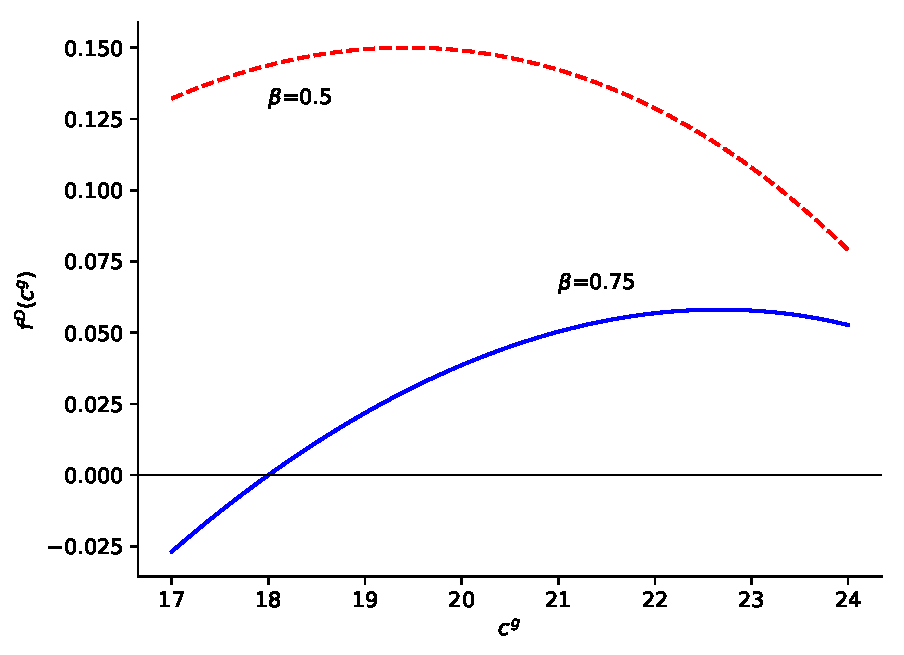
\includegraphics[width=0.75\textwidth]{figures/fd.pdf}
  \caption{Determining $c^g$}\label{fig:fd}
\end{figure}

The variance of the endowment process is less general, but if beta is high enough, increasing the variance of the endowment process (holding the mean fixed) increases the desire for insurance and allows for more risk sharing.

The interest rate can be found in the usual way,
\begin{align}\label{}
 1 + i = \frac{{{c^b}}}{{\beta {c^g}}}.
\end{align}
In the symmetric first best equilibrium, we have $i = {1 \mathord{\left/
 {\vphantom {1 \beta }} \right.
 \kern-\nulldelimiterspace} \beta } - 1$, which is 1 in our numerical example.  In general, if we have not reached the first best we have ${c^g} > {c^b}$ so the interest rate with binding rationality constraints has interest rates lower than in the first best.  In the numerical example it is 0.77.


\subsection*{Stochastic Equilibrium}
Now consider random endowments.  In each period an \textit{event} ${\eta _t} \in \left\{ {1,2} \right\}$ occurs.  The event specifies which agent has the high endowment, ${\omega ^g}$.  Let the probability of a reversal (that is, going from the good to the bad endowment) be $\pi $.  There are two events that can happen in each period, so the Markov transition matrix is two-by-two with elements $\left( {1 - \pi } \right)$ on the diagonal and $\pi $ on the off diagonal.  Define a \textit{history} as the list of events that have occurred, $s = \left( {{\eta _1},{\eta _2},...,{\eta _t}} \right)$.  This history occurs with probability ${\pi _s}$ which is computed in the usual way.

The agent's problem is written as
\begin{align}\label{}
  \max (1 - \beta )&\sum_{s \in S} {{\beta ^{t(s)}}\pi_s \log c_s^j}\\
 \mathrm{s.t.}\;\; \sum_{s \in S} {{p_s}c_s^j} &  \leq \sum_{s \in S} {{p_s}(w_s^j + \theta _0^jr)}\\
 %
 \left(1 - \beta\right)\sum_{\sigma \geq s}\beta ^{t(\sigma ) - t(s)} \left(\pi_\sigma /\pi _s\right) \log c_\sigma^j  &\geq \left( 1 - \beta\right)\sum_{\sigma \geq s} {{\beta ^{t(\sigma ) - t(s)}}\left(\pi_\sigma/\pi _s\right) \log w_\sigma^j}\\
 c_s^j & \geq 0, \;\;\;\theta _0^j = \bar \theta _0^j
\end{align}
Note that I am not using the ``double-sum'' notation to express the stochastic environment.  This is in homage to Kehoe and Levine. The single summation is over all possible histories and the function $t(s)$ returns the period in which the history ends (the length of the history). The summation notation $\sigma \geq s$ means ``all histories $\sigma$ that can be reached from history $s$.''

Solving the stochastic version of this economy is very similar to the deterministic one for the usual reasons.  With complete markets, we just treat goods in different states as different goods and march on.  We are looking for a consumption allocation that has the same form as the one we computed in the  deterministic model.  We can form the analogue of the deterministic ${f^D}({c^g})$ function,
\begin{equation}\label{}
  {f^D}({c^g}) = (1 - \beta (1 - \pi ))\left[ {u({c^g}) - u({\omega ^g})} \right] + \beta \pi \left[ {u(w - {c^g}) - u({\omega ^b})} \right],
\end{equation}
which has the same interpretation.  [to do: show how to derive this.  Write out the recursive formulation, work backwards.]

With the same numbers: ${\omega ^g} = 24$, ${\omega ^b} = 9$, $r = 1$, and $\beta  = 0.5$, plus $\pi  = 0.5$.  Solving ${f^D}\left( {{c^g}} \right) = 0$ yields ${c^g} = 21.52$ and thus ${c^b} = 12.48$.  We can achieve less risk sharing in the stochastic economy.  How does this result vary with changes in the persistence of the endowment, $1 - \pi $?


\section{Unconditional debt and default}
We know from \citet{NP05} (and \cite{uribeYu}) that emerging economies have more volatile business cycles and that $\cor\left(R_t,y_t \right) <0$.  In those models the interest rate was an exogenous process, and the models tried to generate business cycles that were driven by interest rate shocks.

In \citet{A08}, the goal is to endogenize default risk and have it determine country-specific interest rate spreads.  Like  \citet{EG81}, fluctuating endowments generate a desire to smooth consumption by borrowing and lending with the rest of the world.  In contrast to \citet{EG81}, debt in this model is \textbf{non-contingent} and interest rates are endogenous.  The non-contingent debt is key to generating default in states with low output.  Intuitively, long recessions will generate increases in borrowing by the country.  Since debt is non-contingent, staying in the debt contract becomes more painful as the recession continues.  This makes the country more likely to default in low-endowment states. Contrast this to models with contingent debt --- where countries receive pay outs in low-endowment states, and pay back in high-endowment states --- in which default happens in the high-endowment states.

\subsection{The model}

\begin{description}
    \item[Endowments] $y \in [\underline{y}, \bar{y}]$ are stochastic, with Markov transition probabilities $f\left(y'|y \right)$

    \item[Discount bonds] $B'$ with price $q\left(B',y \right)$.  Prices depend on debt and endowments because they affect the default decision. When $B'>0$ the country is saving.  When $B'<0$ the country borrows.  It can choose to repay or default.
    \item[Feasibility (when there is no default)]
    \begin{equation}\label{eq:feas}
        c=y+B-q\left(B',y \right)B'
   \end{equation}

    \item[Default] If a country defaults, debt is discharged.  The country is not able to borrow or lend for a stochastic number of periods: $c=y$.  In default, some of the endowment is lost, $y^{def}=h(y)$, and the amount of this loss depends on the size of the endowment.  We will need that it is more costly to default when endowments are high.

    \item[Creditors] Foreign lenders are risk neutral with a constant cost of funds of $r$. We will have $\beta(1+r)<1$.  Lenders take the $q$ schedule as given and solve
        \[
        \max_{B'} \;\; qB' - \frac{1-\delta}{1+r}B'
        \]
        The object $\delta$ is the probability of the country defaulting.  In equilibrium, it is a function of $(B',y)$.  This is why the bond price is a function of $(B',y)$.

        If $B'>0$ or $\delta = 0$ then $q = \left(1+r \right)^{-1}$. If $B'<0$ or $\delta > 0$ then $q = \frac{1-\delta}{1+r}$.  Bond prices only change to offset default risk --- there is no risk aversion adjustment.

        \[ q(B',y) = \frac{1-\delta\left(B',y \right)}{1+r} \qquad q \in [0,(1+r)^{-1}]
        \]

    \item [The government] The benevolent government maximizes household welfare. The discrete choice is between continuing in the debt contract ($c$) or defaulting ($d$). The timing: observe $y$; choose default or continue; if continue, choose $B^\prime$.

    \begin{align} \label{eq:default_decision}
      v^o\left(B,y \right) = \max_{c,d} \left\{ v^c\left(B,y \right), v^d \left(y \right) \right\}
    \end{align}


    When the country is in default, the government's value is
        \begin{align}
          v^d\left(y \right) = u\left(y^{def} \right) + \beta \int_{y'} \left[\theta v^o\left( 0,y' \right)+\left(1-\theta \right) v^d\left(y' \right)\right]f\left(y'|y \right)dy'
        \end{align}

    where the country consumes its default-penalized endowment until it is let back into the international financial market.  This happens with probability $\theta$. When the government continues in the contract, its value is
    \begin{align} \label{eq:value_continue}
      v^c\left(B,y \right) =\max_{B'} \left \{ u\left(c=y-q\left(B',y \right)B'+B \right) + \beta \int_{y'} v^o\left( B',y' \right)f\left(y'|y \right)dy' \right\}.
    \end{align}

    It is typical to characterize the solution to \eqref{eq:default_decision} as a set of endowments for which the country either defaults or continues
    \begin{align}
      A\left(B \right) &= \left \{ y \in Y: v^c\left(B,y \right) \geq v^d\left(y \right)\right \} \\
      D\left(B \right) &= \left \{ y \in Y: v^c\left(B,y \right) < v^d\left(y \right)\right \}
    \end{align}
    Note that $D$ is the complement of $A$: for a given level of debt, the endowment space is partitioned into two. With the default sets in hand, we can compute the probability of default as
    \begin{align}
      \delta\left(B',y \right) = \int\displaylimits_{D\left(B' \right)} \!\!\! \!f\left(y|y' \right)dy'
    \end{align}
    \item [Equilibrium] Straightforward.  See the paper.
\end{description}

\textbf{Proposition 1}: For all $B_1 \leq B_2$, $D\left(B_2 \right) \subseteq D\left(B_1 \right)$. In words: when the economy borrows more $(B_1)$ there are more states of the world in which it would like to default. Sketch of proof: from \eqref{eq:default_decision} the default cost is the same for both debt levels (no $B$ in the value function), but the continuation value gets smaller as the country borrows more: \eqref{eq:value_continue} is increasing in $B$.

Given this proposition, and that the shocks are bounded above and below, we can define
    \begin{align}
       \underline{B} &= \sup \left \{ B: D\left(B \right) = Y\right \} \\
      \overline{B} &= \inf \left \{ B: D\left(B \right) = \emptyset \right \},
    \end{align}
which says there is a debt level above which you always repay, and one below which you always default.

\subsection{Model with  i.i.d. endowment shocks}
Let's make some simplifying assumptions so that we can prove some theorems. We will use the more general model in the quantitative sections.
\begin{enumerate}[itemsep=0.0ex]
  \item i.i.d. endowments
  \item Excluded from market forever upon default
  \item No output loss in default
\end{enumerate}
If we let the endowment be iid over time, the default decision is no longer dependent on the current realization of the endowment, so policy functions are only a function of bond holdings, $s=(B,y) \rightarrow s=B$.

\textbf{Proposition 2}: If you are at a $B$ such that $D(B) \neq \emptyset$ then the only contracts available require you to pay out, $B-q(B,B')B'<0$.

Intuition: When you have borrowed enough to put the country into the default region, the contract no longer provides an increase in consumption relative to output. Look at \eqref{eq:feas}.  You would never default if there was a contract available that would let you increase your consumption today.  You can always roll over and default later.

\textbf{Proposition 3}: For $y_1 \leq y_2$, if $y_2 \in D(B)$ then $y_1 \in D(B)$.

Intuition: By proposition 2, if $y_2$ is in the default set, then the country is paying back in the next period.  For a given $B$, a lower endowment means lower consumption. Since $u$ is concave, paying back when I am poor hurts more, making me more likely to default.

This is in contrast to many  other models, where the contract doesn't have the country pay out in the low output state.

\textbf{Default space}\\
As long as the country is in the defaultable space $B<\bar{B}$ then the default set is $[\underline{y},y^*(B))$.  See Figure~\ref{fig:dfs}.

\begin{figure}[ht]
\caption{The default region, the iid case.}
\label{fig:dfs}
\centering
\begin{tikzpicture}[xscale=3, yscale=3]
  %\draw[<->] (0,2)--(0,0)--(1.1,0)  node[below]{$k$};
  \draw[<->] (-2,0)--(1,0) node[right]{$B$};
  \draw[->] (0,0)--(0,2) node[right]{$y$};
  \draw[thick]  (-0.5,0.2)  -- (-0.5,0.57) ;
  \node[below] at (-0.5,0){$\bar{B}$};
  \draw[thin] (-0.05,1.8)--(0.05,1.8) node[right]{$\bar{y}$};
  \draw[thick]  (-1.5,1.2)--(-1.5,1.8) node[right]{$y^*(B)$};
  \node[below] at (-1.5,0) {$\underline{B}$};
  \node[right] at (-1,1) {Repay};
  \node[right] at (-1.6,0.7) {Default};
  \draw[thick, domain=-1.5:-0.5] plot(\x, {exp(0.5 - 2*0.5* (\x + 2 ))+0.2} ) ;
  %\draw[-, thick] (0,1)--(1,1) node[right]{$\frac{w_2}{w_1}$};
  %\draw[dashed] (0.5,-0.1) node[below]{$\hat{k}$}--(0.5,1);
  %\node[below, align=left] at (0.25,0) { \footnotesize Country 2 exports\\ \footnotesize these goods};
  %\node[below, align=left] at (0.75,0) {\footnotesize Country 1 exports\\ \footnotesize these goods};
\end{tikzpicture}
\end{figure}


\textbf{Bond prices}\\
The bond price is then
\begin{equation}
    q(B')=\frac{1-F\left(y^*\left(B' \right) \right)}{1+r}
\end{equation}
where $F$ is the CDF of the endowment. This price goes to $1/(1+r)$ when the default probability goes to 0.  See the other hand drawn picture.

\begin{figure}[ht]
\caption{Bond prices, the iid case.}
\label{fig:qb}
\centering
\begin{tikzpicture}[xscale=3, yscale=3]
  %\draw[<->] (0,2)--(0,0)--(1.1,0)  node[below]{$k$};
  \draw[<->] (-2,0)--(1,0) node[right]{$B$};
  \draw[->] (0,-0.1)--(0,2) node[right]{$q(B)$};
  %\draw[thick]  (-0.5,0.2)  -- (-0.5,0.57) ;
  \node[below] at (-0.5,0){$\bar{B}$};
  \draw[thick] (-0.5,1.2)--(0.05,1.2) node[right]{$\frac{1}{1+r}$};
  %\draw[thick]  (-1.5,1.2)--(-1.5,1.8) node[right]{$y^*(B)$};
  \node[below] at (-1.5,0) {$\underline{B}$};
  \draw[thick,<-] (-1.9,0)--(-1.5,0);
  \node[right] at (-1,1) {Todo: connect these two stubs with a concave curve};
 % \node[right] at (-1.6,0.7) {Default};
  %\draw[thick, domain=-1.5:-0.5] plot(\x, {exp(0.5 - 2*0.5* (\x + 2 ))+0.2} ) ;
  %\draw[thick, domain=-1.5:-0.5] plot(\x, { -(\x)^2 +2.25 } );
  %\draw[-, thick] (0,1)--(1,1) node[right]{$\frac{w_2}{w_1}$};
  %\draw[dashed] (0.5,-0.1) node[below]{$\hat{k}$}--(0.5,1);
  %\node[below, align=left] at (0.25,0) { \footnotesize Country 2 exports\\ \footnotesize these goods};
  %\node[below, align=left] at (0.75,0) {\footnotesize Country 1 exports\\ \footnotesize these goods};
\end{tikzpicture}
\end{figure}


Now think about $q(B')B'$. [Figure 2 in the paper]  We know that $q$ is increasing over $(\underline{B},\bar{B})$, but $q(B')B'$ is first decreasing and then increasing.  As we accumulate more debt, we are more likely to default.  This makes the bond price fall more quickly, making $qB$ decrease.  With lower debt levels, the probability of default falls fast enough that $qB$ is increasing.  Note that you would never choose debt on the decreasing part of the curve.


\textbf{Calibration}\\
Table 1: business cycle data.  Looks like \citet{NP05}. The first column is the deviation from trend at time of default. Consumption and output are low, yet the trade balance is positive. Argentina is being asked to pay back during a recession. Column three says that the trade balance is countercyclical. Argentina pays back when times are bad. [\citet{AG07} argue this is the result of trend shocks.] Column four shows that interest rates  are countercyclical: through the lens of the model, the low output periods are greater default periods, so countries pay higher interest rates.


Need to flexibly set $h$ so that the range of risky default, $(B^*, \bar{B})$ (figure 2) is large enough to get some action.  In other words, exclusion alone isn't enough to support enough debt when default is very likely. The form for $h$ suggests that default when the endowment is low doesn't cost anything, but defaulting in good states is increasingly expensive  (equation 13).

Standalone calibration: Take the risk free rate from the U.S. (1.7\%), risk aversion to be 2, and estimate the endowment process from Argentine GDP.  This doesn't include the 2001 default.

Jointly calibrate $\beta$, $\theta$, and $\hat{y}$ to get default probability, debt service-to-gdp ratio (like an interest rate) and trade balance volatility.

Test the model to see if it can account for movements in the interest spread fluctuations and business cycle co-movements.
\subsection*{Model performance}

\textbf{Figure 3}:  The bond price schedule for a high shock and a low shock (In the iid model, this did not depend on $y$). Financial conditions are much better in good times.  This is because shocks are persistent, and countries mostly want to default in bad times.

Panel two is the actual interest rates paid when the country has a given level of debt.  (We are applying the policy function for borrowing, and this is the implied interest rate.)  With a low shock, the country defaults if it had debt levels below --0.02. With a good shock, debt levels below about --0.04 move the country into risky (high rate) borrowing.


\textbf{Figure 4}: the default thresholds are where the value functions go flat.
\begin{enumerate}
  \item Default happens at lower levels of debt in the bad state (about --0.02).
  \item When wealth is high and positive ($B>0.1$) the model behave like a model of commitment. The low-shock savings is below the high-shock savings, generating the consumption smooth motive.
  \item When the country has risky debt, things reverse. Saving is lower in good times than bad times. When times are good, it is easier to borrow, so you borrow more to try and get some from loading of consumption.
\end{enumerate}



\textbf{Table 4}: I wish the data were reported here. Model generates a countercyclical trade balance, even though this is a model of insurance. This means the calibration puts the economy mostly into the risky debt portion of Figure 4.  The countercylicality of interest rates is driving this.  In booms, interest rates are low, so you borrow to tilt consumption towards the future ($\beta(1+r)<1$). When you get a bad shock, interest rates rise and you try to pay back.



\textbf{Risk averse lenders} The model's big miss is on the average spread: 3.58 in the model versus 10.25 in the data.  If lenders are risk averse, then defaults that happens when lenders have a high marginal utility of consumption will drive even larger spreads.

\newpage
\subsection*{Proof of proposition 3}


The gain to defaulting is
\begin{align*}
  \gamma(y_2) =& u(y_2)+\beta Ev^d(y^\prime) - \left[u(y_2+B-q(B^2)B^2)+ \beta Ev^o(B^2,y^\prime)\right]  \\
  \gamma(y_1)= & u(y_1)+\beta Ev^d(y^\prime)-\left[ u(y_1+B-q(B^1)B^1)+ \beta Ev^o(B^1,y^\prime)\right]
\end{align*}


We know that $0<\gamma(y_2)$ since $y_2\in D(B)$. If we can show $0<\gamma(y_2)< \gamma(y_1)$ then we know that $y_1$ is in the default set, too, and that the incentive to default is strictly greater.
\begin{align*}
u(y_2)+\beta Ev^d(y^\prime) -& \left[u(y_2+B-q(B^2)B^2) + \beta Ev^o(B^2,y^\prime)\right] <\\
  &u(y_1)+\beta Ev^d(y^\prime)  - \left[ u(y_1+B-q(B^1)B^1)+ \beta Ev^o(B^1,y^\prime)\right]
\end{align*}

Since endowments are iid we can get rid of $\beta Ev^d(y^\prime)$ to yield
\begin{equation}\label{eq:gain1}
u(y_2) - \left[u(y_2+B-q(B^2)B^2)+ \beta Ev^o(B^2,y^\prime)\right] <  u(y_1)  - \left[u(y_1+B-q(B^1)B^1)+ \beta Ev^o(B^1,y^\prime)\right]
\end{equation}

Because $B^2$ is a maximizer it must be that

\begin{equation*}
  u(y_2+B-q(B^1)B^1)+\beta Ev^o(B^1,y^\prime) \leq u(y_2+B-q(B^2)B^2)+\beta Ev^o(B^2,y^\prime)
  \end{equation*}

so we need to show, since we are subtracting a smaller number from the left hand side of \eqref{eq:gain1},
\begin{align*}
u(y_2) - \left[u(y_2+B-q(B^2)B^2)+ \beta Ev^o(B^2,y^\prime)\right] &\leq \\
  u(y_2) - \left[u(y_2+B-q(B^1)B^1)+ \beta Ev^o(B^1,y^\prime)\right] &<  u(y_1)  - \left[ u(y_1+B-q(B^1)B^1)- \beta Ev^o(B^1,y^\prime)\right]
\end{align*}
which is
\begin{align*}
u(y_2) - \left[u(y_2+B-q(B^1)B^1)+ \beta Ev^o(B^1,y^\prime)\right] &<  u(y_1)  - \left[ u(y_1+B-q(B^1)B^1)- \beta Ev^o(B^1,y^\prime)\right] \\
  u(y_2) - u(y_2+B-q(B^1)B^1) &<  u(y_1)  - u(y_1+B-q(B^1)B^1) \\
  u(y_2) - u(y_1) &< u(y_2+B-q(B^1)B^1)   - u(y_1+B-q(B^1)B^1)
\end{align*}

Since $y_2$ is in the default set for debt level $B$, then the default set is non-empty, and the only contracts available have $B-q(B')B'<0$. (Proposition 2) Then, by strict concavity of the utility function, this last inequality is true.

My intuition for this is that when a country is in the risky debt zone, it must repay (prop 2). Concavity of the utility function means that repaying hurts more at lower levels of endowment. The expected continuation value after default is the same for both endowment levels but paying back hurts more when the country has a low endowment.

\section{Long maturity debt}

All the models we have considered feature single-period debt. In reality, governments (and households) use long maturity debt. Let's see what longer debt does for the model's ability to match the data. What follows is a discussion of \citet{chaterjeeEyigungor}, but other papers on this topic include \citet{hatchondo2009long}.

This paper is basically \citet{A08} with long debt and a slightly different (but important) tweak to the endowment process.

The government's endowment process is
\begin{equation}\label{}
  x_t=y_t+m_t,
\end{equation}
where $y \in Y$ is the usual \textbf{finite state} Markov chain, transition probabilities $F(y,y^\prime)>0$. The tweak is $m \in [-\bar{m}, \bar{m}]$ which is distributed i.i.d. each period with continuous CDF $G(m)$. This extra randomness solves some problems with existence of equilibrium, which we will try and sort out later.

\subsection*{Debt}
Each unit of debt matures in the next period with probability $\lambda$, and needs to be repaid. Each unit that does not mature delivers a coupon $z$. A bond is characterized by a $(\lambda, z)$ pair, which governs the expected maturity and the coupon rate.

This is a tractable way of specifying debt because regardless of when it was issued (one quarter ago, 10 years ago,\ldots) the payoff going forward is the same. This means we only need to track the total amount of debt for each $(\lambda,z)$ bond. Compare this to a bond that pays of deterministically after $K$ periods. This requires tracking $K$ stocks of outstanding debt (how much debt was purchased one quarter ago, 10 years ago\ldots). That's a lot more state variables.

Assume that each bond is infintesimally small, so that a stock of $b$ bonds means that, in the next period, the government owes $\lambda b$ in principle and $(1-\lambda)b z$ in coupon payments.

If the government defaults, three things happen
\begin{enumerate}
  \item Not allowed to borrow or lend until let back into financial markets. With probability $\xi$ it regains access.
  \item The persistent component is penalized $\phi(y)<y$
  \item The iid component is $-\bar{m}$ until let back into the market
\end{enumerate}
The endowment when in default is $x=\phi(y)-\bar{m}$ and parameters are such that $x=\phi(y)-\bar{m}>0$ which means that the endowment is positive for \textbf{any} value of $m$.

%%%%%%%%%%%%%%%%%%%%%%%%%%%%%%%%%%%%%%%%%%%%%%%%%%%%%%%%%%%%%%%%%%%%%%%%%%%%%%%%%%%%%%%%%%%%%%%%%%%%%%%%%%%%%%%%%%%%%%%%%%%%%%%%
\begin{mybox}{Alternative ways to model long bonds}
\citet{hatchondo2009long} model debt as  infinitely-lived bonds that pay an infinite stream of decreasing coupons. [Consols are infinite bonds, but do they have this coupon structure? Need to look into this.]

A bond issued at $t$ pays one unit of the consumption good in $t+1$, and $(1-\delta)^{s-1}$ units of the consumption good in period $t+s$, for all $s=2,3,\ldots$ This is equivalent [I think?] to having the bond pay a unit coupon, but have $\delta$ share of the stock decay away each period. The law-of-motion for coupon payments is
\begin{equation}\label{}
  b^\prime = b(1-\delta)-i
\end{equation}
where $b$ is the number of coupons to pay at the beginning of $t$, $i$ is the issuance of new coupon claims and $b^\prime$ is the stock of coupons to pay in the next period. The government's budget constraint without a default choice is
\begin{equation}\label{}
  c=y+b-q(b^\prime,y)[b^\prime-(1-\delta)b]
\end{equation}

This set up ties together the coupon payment and the maturity of the bond. It is isomorphic to the \citet{chaterjeeEyigungor} bond with $\lambda=1-\delta$ and $z=1$. [Talk about Macaulay duration?]
\end{mybox}
%%%%%%%%%%%%%%%%%%%%%%%%%%%%%%%%%%%%%%%%%%%%%%%%%%%%%%%%%%%%%%%%%%%%%%%%%%%%%%%%%%%%%%%%%%%%%%%%%%%%%%%%%%%%%%%%%%%%%%%%%%%%%%%%%

\subsection*{Lenders}
Lenders are the same as in \citet{A08}. Continuum of risk neutral, deep pocketed, lenders. The price of debt is $q(y,b)$. Notice that the price does not depend on $m$, because it does not help forecast other variables, and thus, default.

\subsection*{Government's problem}
The government makes a discrete choice between default and staying in the contract
\begin{equation}\label{eq:gov-discrete}
  W(y,m,b)=\max \{V(y,m,b),X(y,-\bar{m})\}
\end{equation}

Where $X$ is the value of defaulting,
\begin{align}
  X(y,m)&=u(c)+\beta(1-\xi)\E_{(y^\prime,m^\prime)|y}X(y^\prime,m^\prime)+\beta\xi\E_{(y^\prime,m^\prime)|y}W(y^\prime,m^\prime,0)\\
  c&=y-\phi(y)+m.
\end{align}
The second term on the right hand side of the value function is the expected value of remaining in default and the third term is the expected value of returning to financial markets with $b=0$.

The government makes no decision here. It just eats its endowment and waits.

When the government is in the contract it solves,
\begin{align}
  V(y,m,b)&=\max_{b^\prime}u(c)+\beta\E_{(y^\prime,m^\prime)|y}W(y^\prime,m^\prime,b^\prime)\\
  c&=y+m+\lambda b +(1-\lambda)bz-q(y,b^\prime)[b^\prime-(1-\lambda)b].
\end{align}
\begin{enumerate}
  \item $\lambda b$ = debt that has matured and is due
  \item $(1-\lambda)bz$ = coupon payments on the remaining debt
  \item $q(y,b^\prime)[b^\prime-(1-\lambda)b]$ = the value of the change in the stock of debt
\end{enumerate}
The solution to this problem is a default function $d(y,m,b)$ equal to 1 if default and zero otherwise, and a debt decision rule (when not in default) $b^\prime=a(y,m,b)$.

\subsection*{Debt prices}
Given the lender's characteristics, the debt price is
\begin{equation}\label{eq:ce-price-debt}
  q(y,b^\prime) = \E_{(y^\prime,m^\prime)}\left(1-d\left(y^\prime,m^\prime, b^\prime\right)\right)\frac{\lambda+(1-\lambda)(z+q(y^\prime,a(y^\prime,m^\prime,b^\prime))}{1+r}
\end{equation}
When there is repayment, the lenders receives $\lambda$ units of principle, $(1-\lambda)z$ units of coupon, and the remaining debt revalued at tomorrow's price, $q(y^\prime,a(y^\prime,m^\prime,b^\prime)(1-\lambda)$. [This is where the $a$ functional notation is helpful. Otherwise we would have something like $b^\prime(y^\prime, m^\prime, b^{\prime\prime})$.]

\begin{enumerate}
  \item If debt is one-period, $\lambda=1$ then we are back to \citet{A08}
  \item If the government repays today, but conditions suggest you are more likely to default in the future, $q(y^\prime,a(y^\prime,m^\prime,b^\prime)$ falls, which  decreases the value of debt \textbf{today}. This doesn't happen with short debt.
  \item This is a functional equation in $q$. The bond price enters both through the default probability, the $q$ in the numerator, and through $a$.
\end{enumerate}

\textbf{Proposition 1}: If $b^1 \geq b^2$ then $d(y,m,b^1) \leq d(y,m,b^2)$. More likely to default when you have more debt.

\textbf{Proposition 2}: If $q(y,b^\prime)$ is increasing in $b^\prime$, then $a(y,m,b)$ is increasing in $b$. The ``if'' says that making choosing a more positive debt level brings higher debt prices. On the RHS we have $1-d$, which from prop 1 we know is getting larger when debt is more positive.

\subsection{Technical Issues}
Computing the model equilibrium requires iterating on \eqref{eq:ce-price-debt}. For this to work, the functional equation has to be continuous in $q$. Without $m$ (only a discrete $y$) this is not the case. Without $m$, for some $q(y,b)$ it can be the case that the government is indifferent to defaulting. An infinitesimal change in $q$ will cause a discrete change (either to default or not default) in the RHS of \eqref{eq:ce-price-debt}.  Adding the continuous $m$ eliminates this problem.  This is, presumably, a problem with short debt as well. In \citet{A08} theory model, the endowment is assumed to be continuous.

The above issue is an existence problem. Lots of papers use continuous models to prove existence and then go discrete for computation. The authors claim that this is a problem, too. I do not have a handle on this.

\subsection{Quantitative results}
Calibrate to Argentina.

\textbf{Tables 1, 2, and 3.} Take $\sigma_m=0.003$ as being large enough to make the model converge easily, but otherwise small. Set $\bar{m}=2\sigma_m$. Estimate $\rho$ and $\sigma_\epsilon$ from real GDP and then make a discrete approximation.

Set $\lambda=1/20$ to match the median maturity of 20 quarters. Set $z=0.03$ to match an annual coupon of 12 percent. The risk-free rate is 0.01 to match U.S. Treasury yields.

Set $\zeta=0.0385$ so that default leads to exclusion of 6.5 years which is a reasonable approximation to the data.

The last three parameters $\beta$, $d_0$ and $d_1$ are set to jointly match the 1) average spread, 2) the standard deviation of the spread, and 3) the debt-to-GDP ratio. [For measurement reasons, they match b/y to 0.7 rather than 1.0 as in the data. Worth sorting out at some point.] The default penalty function is
\begin{equation}\label{eq:ce-cost-function}
  \phi(y)=\max\{0,d_0y+d_1y^2\}.
\end{equation}

\textbf{Results}\\
In general, the long-bond model does a good job accounting for the data.
\begin{enumerate}
  \item Figure 3: Feed in endowment shocks that match the endowment in Argentina over the period and set the debt level in 1993 to match Argentina. The model and data look good. Compare to \citet{A08} figure 5. This model can generate volatile spreads.

  \item Table 3, last column: These are moments targeted by CE and not by Arellano. This table highlights the moments the one-period debt model couldn't capture. [Could you calibrate Arellano's model to these moments?]

  \item Table 4: The model generates countercyclical spreads and net exports. As in Arellano, this is the result of the default probabilities moving debt prices around in response to the cycle.
\end{enumerate}

When the model is calibrated with one-period debt, the fit to the data is much worse. Table 4: In particular consumption and net exports are much more volatile.
\begin{enumerate}
  \item With one-period debt, the government has to refinance the entire debt stock each period. As $q(y,b)$ moves around, the cost of doing so moves around and so consumption and net exports become very volatile. Note that this is not a big problem in Arellano's model because that model has $b/y=0.06$ compared to $b/y=0.7$ in this paper.
  \item With multi-period debt, the government only owes $[\lambda+(1-\lambda)z]b$ each period and only needs to refinance $\lambda b$ to keep its debt level constant. Movements in $q(y,b)$ require smaller movements in consumption compared to the one-period debt model.
\end{enumerate}

\textbf{The default cost function's role}\\
The default cost function is very important. It is a bit worrisome that an ad hoc bit of the model drives so much of the model's interesting behaviors. [This is not unique to this model or to long-term debt models. I might want to move this somewhere else.]
\begin{enumerate}
  \item The asymmetry in the cost function is important for generating default. When times are good (which is persistent) it is very costly to default, so spreads are low and impatient governments borrow. When output falls (also persistent), the cost of defaulting falls, spreads rise and default is likely to occur.

      If the cost function was symmetric (say, proportional to output) then the cost of default doesn't change much, the spreads stay high, and governments do not accumulate much debt. Low debt levels mean governments rarely default.

  \item The cost function also matters for the volatility of spreads. $d_2$ in \eqref{eq:ce-cost-function} controls the sensitivity of costs to $y$. Table 5: change $d_1$ but recalibrate to keep the other two moments fixed. Spreads increase.

      As spreads become more volatile, the desire to default increases. To keep the government willing to hold $b/y=0.70$, it must be more patient. $\beta$ rises with $d_1$.

      To keep the average spread constant $d_0$ falls. See figure \ref{fig:ce-default-cost}. To keep the average right, the larger punishment at good times is offset by smaller punishments in bad times.
\end{enumerate}
\begin{figure}
  \centering
  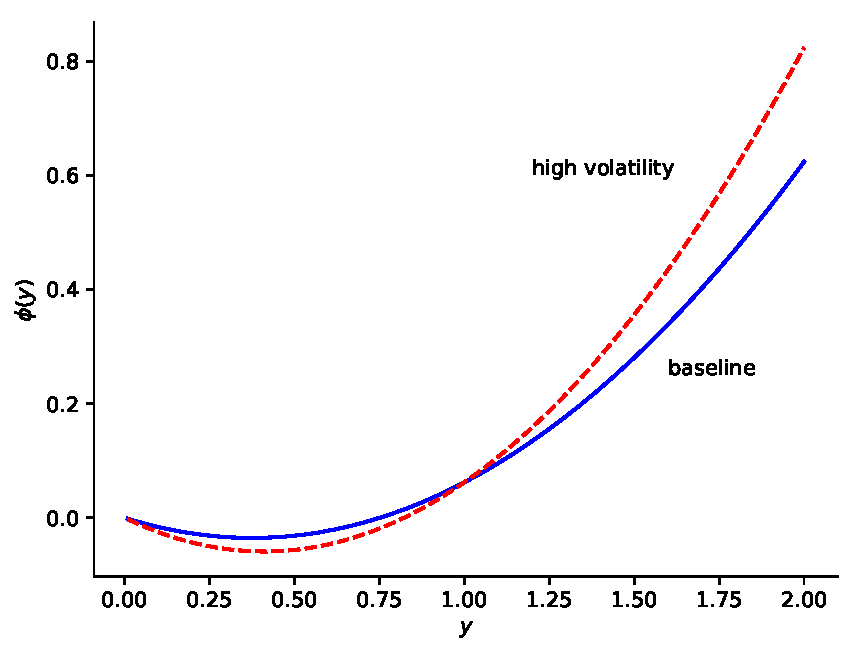
\includegraphics[width=0.7\textwidth]{figures/phi.pdf}
  \caption{The default cost function}\label{fig:ce-default-cost}
\end{figure}
\textbf{Debt dilution}\\
\textit{Debt dilution} is the reduction in the value of existing debt triggered by the issuance of new debt. By issuing more debt today, the government is more likely to default in the future. Table 7: Moving from short-term debt to long-term debt decreases welfare. This is evident in \eqref{eq:ce-price-debt}. The price of all the outstanding debt appears on the right hand side.

There are two effects at work: 1) short term debt makes consumption more volatile, which reduce welfare 2) short term debt has lower spreads because debt dilution risk is eliminated.

In this parameterization, the lower borrowing costs win out. See \citet{hatchondo2016debt} for more on dilution.

\setstretch{1.0}
\setlength{\parskip}{0.0cm}
\printbibliography

\end{document}
